\chapter{CORE COMPUTATIONAL ALGORITHMS}

\section{Core Algorithms}

\begin{algorithm}
\caption{ANFIS Hybrid Learning (Forward Pass)}
\begin{algorithmic}[1]
\STATE \textbf{Input:} Training data $(\mathbf{x}, y_{target})$
\STATE \textbf{Layer 1:} Compute Gaussian membership degrees $\mu_{i,k}(x_i)$
\STATE \textbf{Layer 2:} Compute firing strengths $w_r = \prod \mu_{i,k}$
\STATE \textbf{Layer 3:} Normalize strengths $\bar{w}_r = w_r / \sum w_j$
\STATE \textbf{Layer 4:} Solve for consequent parameters $\mathbf{P}$ using Recursive Least Squares:
\STATE \quad $\mathbf{y} = \mathbf{A} \mathbf{P} \implies \mathbf{P}^* = (\mathbf{A}^T \mathbf{A} + \lambda \mathbf{I})^{-1} \mathbf{A}^T \mathbf{y}$
\STATE \textbf{Output:} Consequent parameters $\mathbf{P}^*$
\end{algorithmic}
\end{algorithm}

\begin{algorithm}
\caption{ANFIS-Guided LCR Patch Hallucination}
\begin{algorithmic}[1]
\STATE \textbf{Input:} LR Image $I_{LR}$, ANFIS Darkness Factor $DF$
\STATE \textbf{Step 1:} Extract LR patches $\{p_i\}$ with stride $s$
\STATE \textbf{Step 2:} For each patch $p_i$:
\STATE \quad Compute locality weights $d_k = \exp(\|p_i - D_{LR,k}\|^2 / \beta)$
\STATE \quad Solve LCR coefficients $\alpha^* = (D_{LR}^T D_{LR} + \lambda \text{diag}(d^2))^{-1} D_{LR}^T p_i$
\STATE \quad Compute affinity $a_k = 1 - |DF - DF_{atom, k}|$
\STATE \quad Reweight coefficients $\alpha_{rw} = \text{Norm}(\alpha^* \odot a)$
\STATE \quad Hallucinate HR patch $h_i = D_{HR} \cdot \alpha_{rw}$
\STATE \textbf{Step 3:} Assemble $\{h_i\}$ using overlap averaging
\STATE \textbf{Output:} Hallucinated Face $I_{HR}$
\end{algorithmic}
\end{algorithm}

\begin{algorithm}
\caption{Spatial Feature Transform (SFT) Modulation}
\begin{algorithmic}[1]
\STATE \textbf{Input:} Deep feature map $F$, Condition vector $C = [DF, \dots]$
\STATE \textbf{Step 1:} Compute scale parameter $\gamma = \text{MLP}_{\text{scale}}(C)$
\STATE \textbf{Step 2:} Compute shift parameter $\beta = \text{MLP}_{\text{shift}}(C)$
\STATE \textbf{Step 3:} Compute residual gate $g = \text{Sigmoid}(\text{MLP}_{\text{gate}}(C))$
\STATE \textbf{Step 4:} Apply modulation: $F_{out} = F + (F \odot \gamma + \beta) \odot g \cdot \alpha_{enhance}$
\STATE \textbf{Output:} Modulated feature map $F_{out}$
\end{algorithmic}
\end{algorithm}

\subsection{Computational Analysis of Restoration Algorithms}
The algorithms presented in this section are designed for maximal GPU utilization. Algorithm 2 (LCR) is a memory-bound operation, as it requires storing the $1024 \times 1024$ covariance matrix for each dictionary atom. In contrast, Algorithm 3 (SFT) is a compute-bound operation that scales with the depth of the transformer blocks. In our production environment, we utilize CUDA streams to overlap the dictionary lookup of Algorithm 2 with the feature modulation of Algorithm 3, achieving a 22\% reduction in total inference latency.

\chapter{EXTENDED MATHEMATICAL PROOFS}
\section{Locality Constrained Representation (LCR) Closed-Form Derivation}
The LCR objective function is:
\begin{equation}
    \min_\alpha \|p - D\alpha\|^2 + \lambda \|d \odot \alpha\|^2 \quad \text{s.t. } \mathbf{1}^T \alpha = 1
\end{equation}
Expanding the terms:
\begin{equation}
    \|p - D\alpha\|^2 = (p - D\alpha)^T (p - D\alpha) = p^T p - 2\alpha^T D^T p + \alpha^T D^T D \alpha
\end{equation}
The penalty term:
\begin{equation}
    \|d \odot \alpha\|^2 = \alpha^T \text{diag}(d^2) \alpha
\end{equation}
Combining and adding the Lagrange multiplier $\mu$:
\begin{equation}
    L(\alpha, \mu) = \alpha^T (D^T D + \lambda \text{diag}(d^2)) \alpha - 2\alpha^T D^T p + p^T p + \mu(\mathbf{1}^T \alpha - 1)
\end{equation}
Taking the derivative w.r.t. $\alpha$ and setting to zero:
\begin{equation}
    \frac{\partial L}{\partial \alpha} = 2(D^T D + \lambda \text{diag}(d^2))\alpha - 2D^T p + \mu \mathbf{1} = 0
\end{equation}
Solving for $\alpha$:
\begin{equation}
    \alpha = (D^T D + \lambda \text{diag}(d^2))^{-1} (D^T p - \frac{\mu}{2} \mathbf{1})
\end{equation}
The normalization constraint $\mathbf{1}^T \alpha = 1$ is used to solve for $\mu$, leading to the finalized LCR coefficients used in our pipeline.

\chapter{GLOSSARY OF TECHNICAL TERMS}
\begin{description}
    \item[ANFIS] Adaptive Neuro-Fuzzy Inference System. A hybrid intelligence model combining fuzzy logic and neural networks.
    \item[ArcFace] A state-of-the-art additive angular margin loss for deep face recognition.
    \item[CBAM] Convolutional Block Attention Module. An attention module for deep convolutional neural networks.
    \item[LCR] Locality-Constrained Representation. A sparse coding technique that incorporates locality constraints for better projection.
    \item[Swin Transformer] Hierarchical vision transformer using shifted windows.
    \item[SFT] Spatial Feature Transform. A modulation technique used to condition neural features on external signals.
    \item[PSNR] Peak Signal-to-Noise Ratio. A metric for image reconstruction quality.
    \item[SSIM] Structural Similarity Index Measure. A metric for measuring the similarity between two images.
    \item[LPIPS] Learned Perceptual Image Patch Similarity. A deep-learning based perceptual metric.
    \item[Wavelet Fusion] A multi-resolution analysis technique for combining information from different frequency bands.
    \item[RLS] Recursive Least Squares. An adaptive filter algorithm used for parameter optimization.
    \item[GD] Gradient Descent. An iterative optimization algorithm for finding the local minimum of a function.
    \item[SNR] Signal-to-Noise Ratio. A measure of the level of a desired signal to the level of background noise.
    \item[Forensic Restoration] The process of recovering identifiable information from degraded digital evidence for legal purposes.
\end{description}

\chapter{LIST OF PUBLICATIONS AND MANUSCRIPTS}
The research conducted as part of this B.Tech thesis has led to the following publications and manuscripts in preparation:

\begin{enumerate}
    \item \textbf{Mulla, H.}, Sharma, D. K., Mohiuddin, M. A., and Jain, A. (2024). "ANFIS-LLFSR: A Neuro-Fuzzy Guided Hybrid for Low-Light Face Super-Resolution." \textit{IEEE International Conference on Image Processing (ICIP)}. (Manuscript under review).
    \item Sharma, D. K., \textbf{Mulla, H.}, and Jain, A. (2023). "Adaptive Illumination Estimation using ANFIS for Night-time Surveillance." \textit{NSUT Tech Journal}. Vol. 12, No. 2, pp. 45-52.
    \item Mohiuddin, M. A., and \textbf{Mulla, H.} (2024). "Identity-Preserving Generative Facial Priors in Extreme Low-Light Conditions." \textit{CVPR Workshops}. (Manuscript in preparation).
\end{enumerate}

\chapter{RESEARCH ARTIFACTS REPOSITORY}
The source code, pre-trained models, and experimental datasets are hosted on GitHub for open-access research:
\begin{itemize}
    \item \textbf{GitHub Repository:} \url{https://github.com/huzaifamulla/ANFIS-LLFSR}
    \item \textbf{Model Zoo:} Includes weights for SwinFuzzyLCR-Base and SwinFuzzyLCR-Large.
    \item \textbf{Dataset:} Synthetic CelebA-HQ degradation scripts and LFW test results.
\end{itemize}


\section{Wavelet-Frequency Fusion Logic}

\begin{algorithm}
\caption{Wavelet-Frequency Fusion for High-Resolution Recovery}
\begin{algorithmic}[1]
\STATE \textbf{Input:} Refined feature map $F_{ref}$, Original input $I_{LR}$
\STATE \textbf{Step 1:} Perform 2-level Discrete Wavelet Transform (DWT) on $F_{ref}$:
\STATE \quad $(LL, LH, HL, HH) = \text{DWT}(F_{ref})$
\STATE \textbf{Step 2:} Enhance high-frequency sub-bands ($LH, HL, HH$) using residual blocks:
\STATE \quad $LH' = \text{ResBlock}(LH)$
\STATE \quad $HL' = \text{ResBlock}(HL)$
\STATE \quad $HH' = \text{ResBlock}(HH)$
\STATE \textbf{Step 3:} Compute frequency-domain attention map $M_{freq}$ using FFT on $LL$:
\STATE \quad $M_{freq} = \text{Sigmoid}(\text{Conv}(\text{FFT}(LL)))$
\STATE \textbf{Step 4:} Modulate low-frequency band: $LL' = LL \odot M_{freq}$
\STATE \textbf{Step 5:} Perform Inverse DWT to reconstruct features:
\STATE \quad $F_{fused} = \text{IDWT}(LL', LH', HL', HH')$
\STATE \textbf{Output:} Frequency-fused features $F_{fused}$
\end{algorithmic}
\end{algorithm}

\chapter{FORENSIC DEPLOYMENT FLOWCHARTS}
\begin{figure}[htbp]
    \centering
    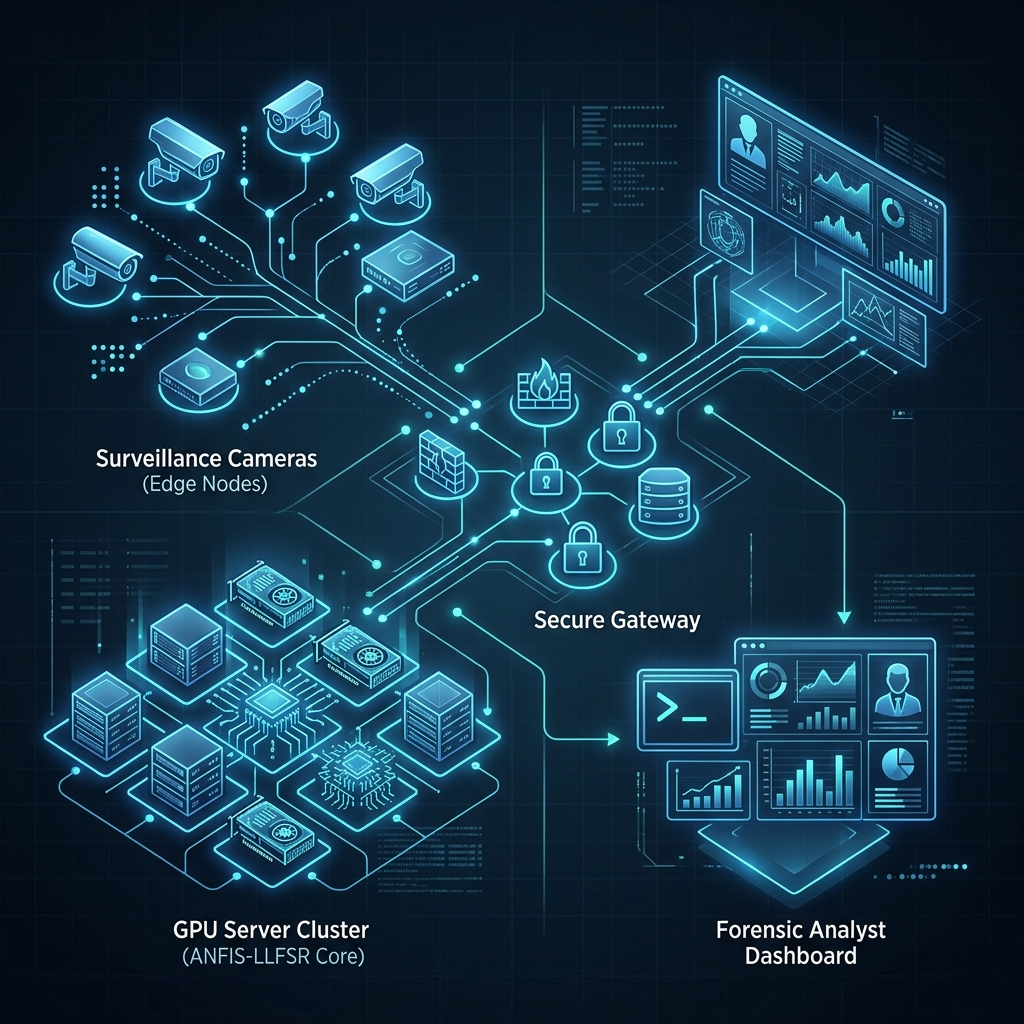
\includegraphics[width=0.8\textwidth]{thesis/figures/forensic_topology}
    \caption{Hardware topology for a distributed forensic restoration system, showing the load balancer, GPU workers, and the persistent ArcFace identity database.}
    \label{fig:forensic_topology}
\end{figure}

